
In \cite{Gardel} Gardel et.al. a method of head detection from above based on circle detection is proposed. In their approach circles, i.e. heads, are detected by first performing canny edge detection on each image frame and then performing a form of hough voting to detect circles. The hough voting is done by combining the results of a series of different filters designed to give high responses at circle and ellipse centers. We implemented their approach and experimented with many different variations of filter sizes and canny variables, with both types of circle filters described in the paper. We also tried using background subtraction on the canny image, using a mixture of Gaussian-based foreground segmentation \cite{Zivkovic} of the raw image, which gave slightly better results in simple situations. We were however not able to get any usable results for anything but the simplest cases, and therefore gave up on this approach after many fruitless attempts at tuning the system. Outputs from some of the different steps of cases where the approach was both successful and unsuccessful can be seen in figure \ref{fig:circle_success} and \ref{fig:circle_fail} below.
\vspace{1cm}
\begin{figure}[htb]
	\centering
	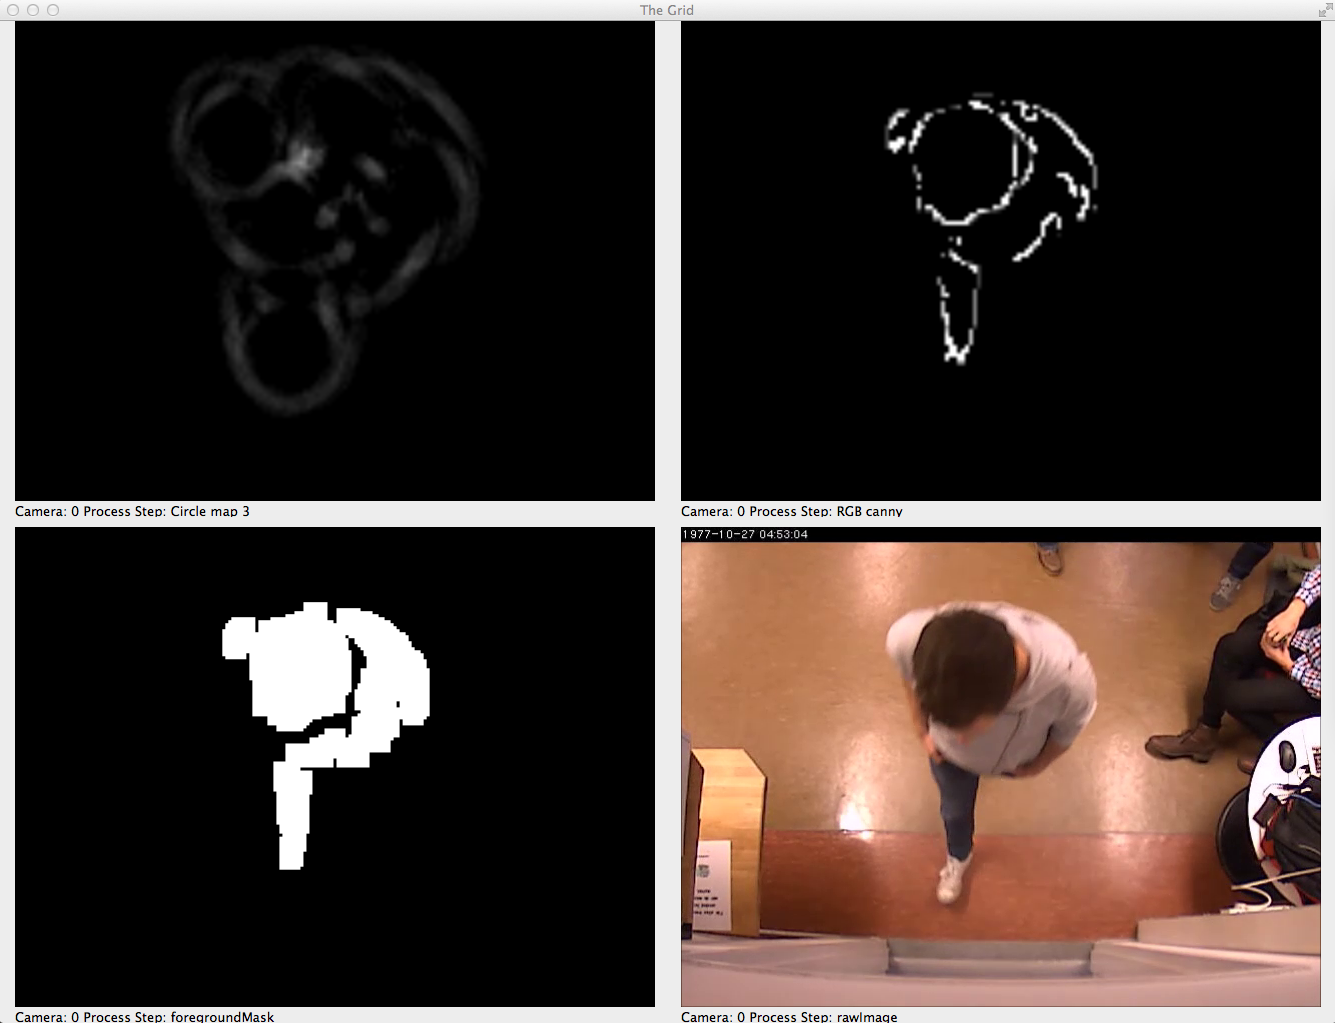
\includegraphics[width=\linewidth]{images/circle_detection_success.png}
	\caption[An example of a successful Hough-circle detection]{\\\textit{
	Top left: output from one of the circle filters.\\ 
	Top right: output from the canny edge detection after background subtraction.\\ 
	Bottom left: foreground mask.\\ 
	Bottom right: raw image.}}
	\label{fig:circle_success}  %Skapar referens till figuren
\end{figure}
\newpage
\begin{figure}[htb]
	\centering
	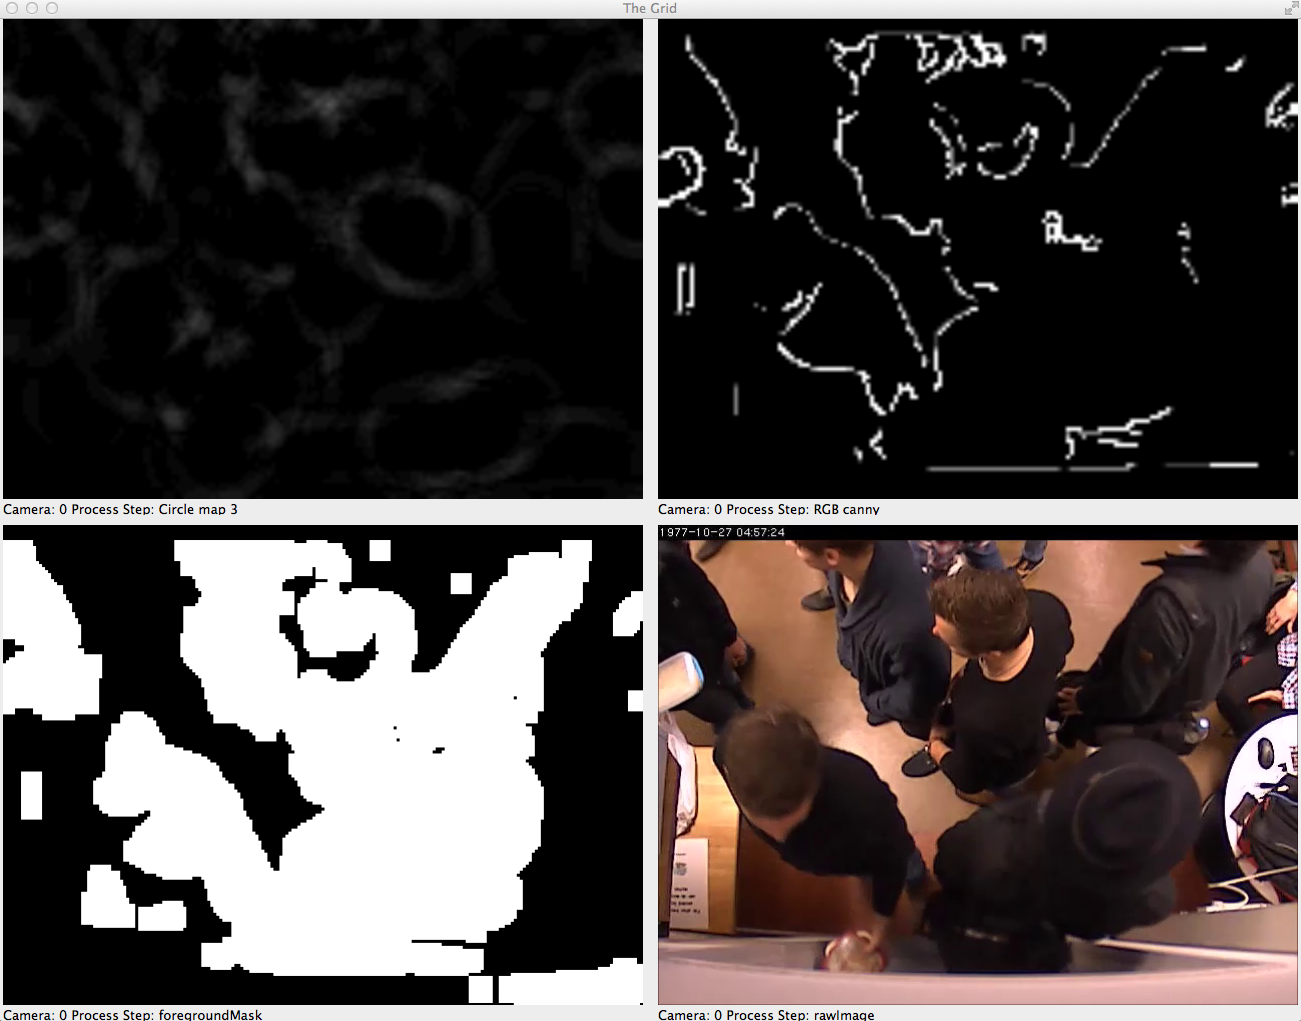
\includegraphics[width=\linewidth]{images/circle_detection_fail.png}
	\caption[An example of a failed Hough-circle detection]{\textit{\\
	Top left: output from one of the circle filters.\\
	Top right: output from the canny edge detection after background subtraction.\\
	Bottom left: foreground mask. \\
	Bottom right: raw image.}}
	\label{fig:circle_fail}  %Skapar referens till figuren
\end{figure}

